%!TEX TS-program = xelatex
%!TEX encoding = UTF-8 Unicode

% Load Thesis Class
\documentclass{DEIThesis}

\title{Scheduling resources and managing HARQ retransmissions in Non-Terrestrial Networks}

\author{Francesco Rossato}
\studentId{2082121}

% Advisor
\advisor{Professor Michele Zorzi}

% If you are co-advised
\coadvisor{Prof.\ Marco Giordani}
\coadvisorsUniversity{University of Padova}
\cocoadvisor{Dr. Matteo Pagin}
\cocoadvisorsUniversity{University of Padova}

\university{University of Padova}
\mastername{ICT for Internet and Multimedia}
\academicYear{2023/2024}

\begin{filecontents*}[overwrite]{\jobname.xmpdata}
    \Title{Simulation Study, Design and Implementation of 5G NR Layer-2 Protocols for Non-Terrestrial Networks}
    \Author{Francesco Rossato}
    \Language{en-EN}
    \Keywords{ntn\sep 5G\sep non terrestrial networks \sep francesco rossato\sep HARQ\sep scheduler\sep layer 2}
\end{filecontents*}

% Document

\begin{document}
    % The front matter (Cover, ToC, Abstract, etc...)
    \frontmatter

    % The main content
    \mainmatter
    %!TEX root = ../main.tex

\chapter{Introduction}
\label{chp:intro}

The term \ac{NTNs} denotes a category of networks where at least one link is routed via an aerial or space-borne vehicle such as \ac{HAPs}, \ac{UAVs} or telecommunication satellites.

\section{The focus on non-terrestrial networks}
The Third Generation Partnership Project \footnote{\href{https://www.3gpp.org}{\texttt{3gpp.org}}} (3GPP), the standardization body developing protocols for mobile communication networks, recently put a great emphasis on the importance of the integration of different access technologies along with the existing terrestrial mobile telecommunication infrastructure \cite{3gpp-tr-21.917}.

The envisioned future for mobile communications, starting with the already established 5G \ac{NR} and expanding with the new sixth-generation cellular networks (6G), foresees the integration of a non-terrestrial component. The latest \ac{3GPP} releases (Rel. 17 and Rel. 18) require 5G and 6G networks to be able to provide non-terrestrial satellite access complementing the already existing terrestrial access technologies \cite{overview-rel-17-18-saad} \cite{5g-nr-communication-geo-leo-maattanen}.

\section{Limitations of terrestrial networks}
The following paragraphs present a few scenarios where terrestrial networks have some limitations, and \ac{NTNs} can be used to provide connectivity.

\subsection{Remote places}
While \ac{TN} make the well-established foundation of today’s mobile communication infrastructure, their own nature poses some intrinsic limitations to their deployment in certain scenarios, especially in rural and remote areas. Conditions such as harsh terrain and geographical impediments act as natural barriers to the deployment of terrestrial infrastructure. Moreover, ground infrastructure requires the presence of an already established reliable power grid, driving up the costs that telecommunication companies would have to sustain.
The population density is often low in remote and rural places, so the already high infrastructure cost will hardly pay for itself, making this kind of market even more unattractive to private investors and further limiting the possibility for the people living there to access a resource which is becoming increasingly more important.

As studied and documented in \cite{6g-challenge-opportunity-base-pyramid}, the issue of an inadequate broadband coverage in rural regions is an enormous challenge, but also a great opportunity to kick-start the economy of currently underdeveloped countries, promoting a more fair access to the internet and alleviating the problem of digital divide between different parts of the world.

\subsection{Redundancy}
Another limitation of the current terrestrial infrastructure is the lack of redundancy and robustness against natural disasters. Extreme events such as earthquakes, fires and floods, but also deliberate behaviors such as targeted attacks by terrorist organizations and sabotages can disrupt the connectivity even for a long period of time, causing significant economical damage and hindering the already difficult rescue efforts, potentially leading to loss of lives.

The simple installation of a greater number of base stations is not a viable solution because they all share the same weaknesses.

In this scenario, \ac{NTNs} can act as redundant access methodology to decrease downtimes of terrestrial infrastructure, provide emergency communication services and also additional capacity when required. 

\subsection{Long distances and sensors}
Remote equipment, offshore plants and distribution grids will also benefit from the research carried out in this field, since providing terrestrial connectivity in those scenarios is a challenging task. The installation of an underwater optical fiber link to serve a single endpoint, such as an offshore power plant in the ocean, would bear a disproportional cost compared to the functions required, and maintenance would be another challenging and expensive task. 
The deployment of a non-terrestrial network would provide connectivity on a global scale, therefore allowing internet access in isolated places without the need for a dedicated connection.

Consider now the problem of connecting of a number of sensors placed in a large area. When distances are large, solutions may either be the densification of radio stations or the use of a lower frequency in order to have a less severe propagation loss. However, those approaches have their downsides and are not always feasible. In this case, the large coverage area of \ac{NTNs} will undoubtedly be useful to provide internet connection \cite{performance-ntn-support-iot-wang}.

\paragraph{} Other scenarios where \ac{NTNs} can become useful in overcoming the limitation of their terrestrial counterpart are well described in \cite{ntn-6g-era-challenges-giordani} and \cite{potential-multilayered-nierarchical-ntn-wang}.

\section{Satellite types}
Satellites are divided in three different categories depending on their orbiting altitude: \ac{GEO}, \ac{MEO} \ac{LEO} satellites. Each one has its own characteristics, as briefly described below.

\subsection{GEO satellites}
orbiting at 35.786Km, \ac{GEO} satellites appear stationary since their orbiting period is the same as the Earth rotation period. This vastly simplifies the tracking for the ground equipment, since once the position of the \ac{UE} is known, the relative position of the satellite is known, too.
    
Since \ac{GEO} satellites are geostationary, continuous coverage to a designated area can be provided using as little as a single satellite, while the use of non-\ac{GEO} satellites would require the deployment of a constellation, which is both more complex and more expensive.

Their higher altitude creates a large cell footprint, larger than both \ac{MEO} and \ac{LEO}, so the overall cost to provide coverage to the same area is lower.

The disadvantages of \ac{GEO} satellites are mainly linked to the large distance with the \ac{UE}: the transmission power and the antenna gain have to be higher to account for the greater propagation losses, and the propagation delay of the signal travelling at the speed of light is about 120ms, so if the \ac{UE} sends a request to a server at time zero through a \ac{GEO} link, the best-case delay will be of half a second without considering any protocol-related delay.

In addition to the positive aspects previously discussed, the larger cell footprint also means that a single satellite will be serving a massive number of users, so the total available capacity will have to be shared between a bigger number of actors, and the throughput experienced by each one of them will be reduced. 
Moreover, the high number of users leads to a large rate of initial access  requests, with the possibility of channel saturation as described in \cite{3gpp-tr-38.811}.

\subsection{LEO satellites}
Orbiting below the altitude of 2.000Km, \ac{LEO} satellites are the most promising solution in the realm of \ac{NTNs} for a number of reasons hereby discussed.
    
The lower altitude entails a shorter propagation delay, and the smaller coverage area of each satellite means that the total number of users that need to be served is smaller. 

The cost per satellite is significantly smaller than \ac{GEO} and \ac{MEO} satellites. However, given that they are not geostationary, a large constellation is needed to provide a continuous service, driving up the deployment costs significantly. As an example of those constellations, Fig. \ref{fig:starlink_constellation} depicts the \ac{LEO} satellites employed by Starlink\footnote{Starlink is a satellite internet constellation operated by Starlink Services, LLC, a wholly-owned subsidiary of American aerospace company SpaceX.}, with 4.808 units in service at the time of writing\footnote{Source: \href{https://satellitemap.space/}{\texttt{satellitemap.space}}}.

\begin{figure}[ht]
    \centering
    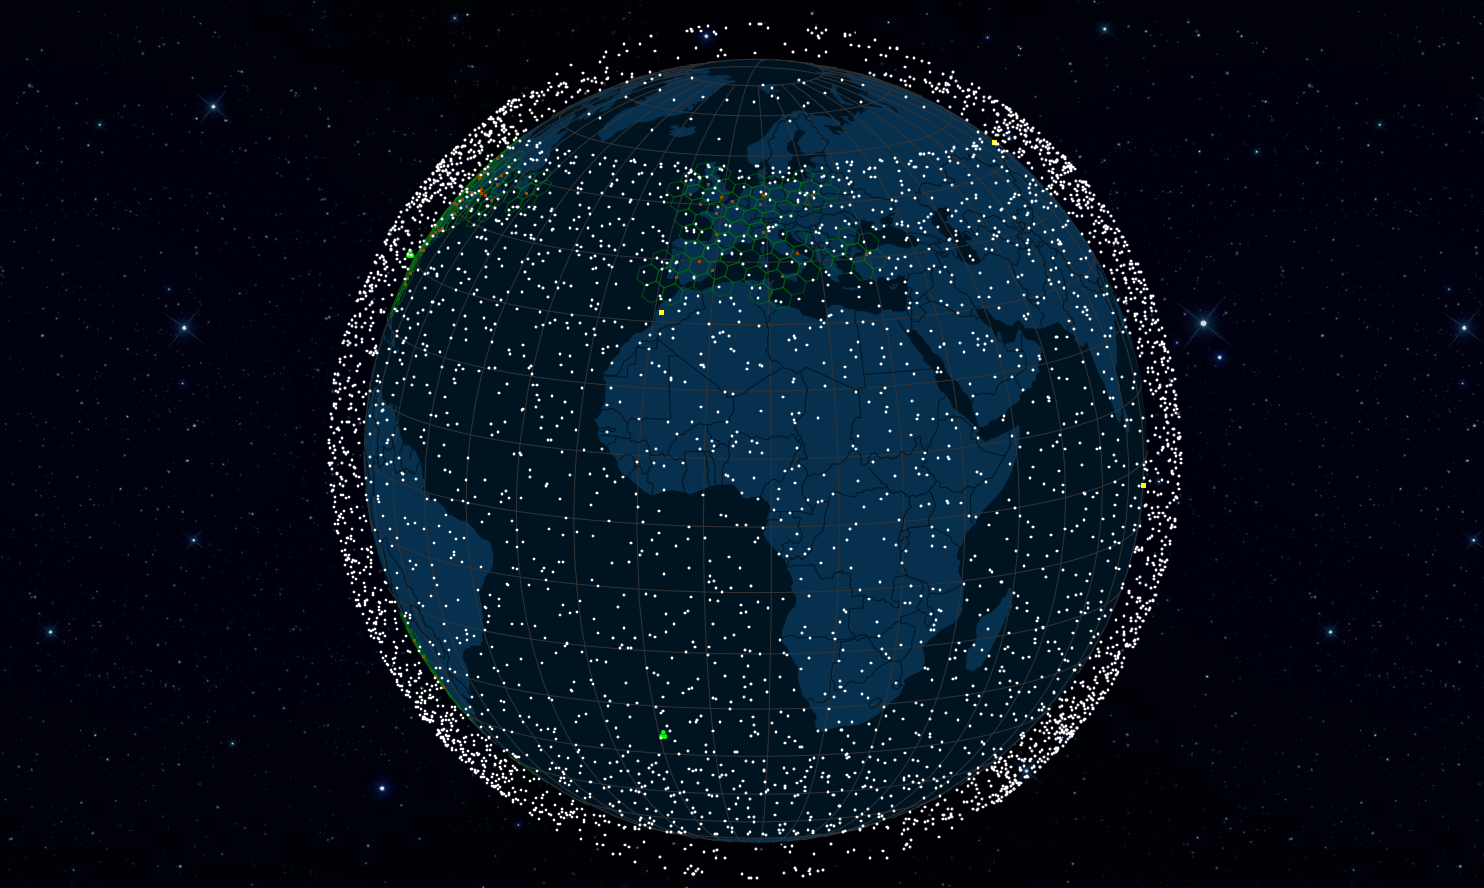
\includegraphics[width=0.7\textwidth]{res/starlink-constellation.png}
    \caption{Starlink constellation as July 2024. Source: \href{https://satellitemap.space/}{\texttt{satellitemap.space}}}
    \label{fig:starlink_constellation}
\end{figure}

The smaller altitude at which \ac{LEO} satellites orbit enables the use of higher frequency bands, since the experienced path loss is smaller compared to \ac{GEO} satellites. This in turn allows for higher throughput, as detailed in \cite{satellite-communication-mmwave-giordani}

The aforementioned solutions are not to be considered mutually exclusive. In fact, the multitude of possibilities that their combinations offer open to the study of various different scenarios, as detailed in \cite{potential-multilayered-nierarchical-ntn-wang}

\subsection{Current solutions}
Current solutions for non-terrestrial communication do exist, but they mostly rely on telecommunications satellites placed in the \ac{GEO}, at a height of 35.786 km. The distance that the signal has to travel offering limited throughput and large delays. While \ac{LEO} constellations (400 km to 2.000 km) have proven to be a valid alternative, providing higher throughput and lower latency \cite{main-features-5g-nr-ntn-yun}, they have the drawback of an increased Doppler shift due to their high speed relative to ground \cite{satellite-communication-mmwave-giordani}, and there is still no international standard with regard to the communication protocols to use. 

\paragraph{}
This scenario led \ac{3GPP} to identify some work to be done to integrate \ac{NTN} in cellular standards, calling for long-term research in this field \cite{satellite-communication-mmwave-giordani}. This work will mainly focus on the 

\paragraph{}\todo{move this to state of the art} Focusing on the \ac{MAC} sublayer, the large propagation delay of satellite links affects different aspects, making the actual implementation not suited for a \ac{NTN} scenario. In the \ac{HARQ} protocol, the retransmission timeout is likely to expire before a single \ac{RTT}, leading to unnecessary retransmissions. Moreover, the limit on the maximum number of concurrent \ac{HARQ} processes leads to a stop-and-wait behaviour, which may increase the energy consumption \cite{3gpp-tr-38.811}. On the other hand, it has been noted that disabling \ac{HARQ} would lead to an even worse performance penalty, therefore requiring a redesign for \ac{NTN} \cite{5g-beyond-5g-ntn-trends-vanellicoralli}. Another 5G \ac{NR} protocol which is negatively impacted in \ac{NTN} is the initial access, since users at the center of the cell face a smaller propagation delay with respect to users at the cell edge \cite{5g-beyond-5g-ntn-trends-vanellicoralli} \cite{applying-nr-technologies-in-ntn-lee}. As a result, preambles of \ac{UE}s placed near the cell edge may reach the satellite when the \ac{RACH} opportunity has already expired, which may lead to collisions. During the initial access phase, \ac{UE}s are not aware of their propagation delay, and the high mobility of \ac{gNB}s on \ac{LEO} satellites causes a non-negligible Doppler shift. Those factors vary with the relative position and speed between the \ac{UE} and the \ac{gNB}, and the protocols for initial access must be modified in \ac{NTN} to account for them \cite{ntn-from-5g-6g-hassan}. 
\paragraph{}
It is clear that the future of mobile networks envisioned by \ac{3GPP} embraces \ac{NTN}s, and considerable work has to be done. Research will bear a high impact towards a more connected, equal opportunity world. 

\section{Currrent state of the art}
\todo{types of payloads: regenerative, and transparent or bent pipe}
    % %!TEX root = ../main.tex

\chapter{State of the Art}
\label{chp:stateOfArt}

\begin{figure}[ht]
    \centering
    
\includegraphics[width=0.5\textwidth]{res/ltunipd}
    \caption{Example of image}
\end{figure}
    %!TEX root = ../main.tex

\chapter{Scheduling problems}
\label{chp:scheduling_problems}

Before starting to tackle the problems that the high propagation delay causes to the \ac{HARQ} protocol, attention shall be put on the random access procedure and on the scheduler, both happening at a lower level, therefore necessary to be able to receive packets.

If those layers are not in working conditions, the communication will not be able to take place.

\section{5G scheduler}
As the name suggests, the main task of the scheduler is to allocate resources to the various connected users in the form of transmission and reception opportunities. In mobile communication networks, the scheduling is dictated by the network and the \ac{UE} has to follow the provided indications.

\subsubsection{5G channels}
The \ac{NR} standard comprises the usage of several channels depending on the type of data to be sent. The medium access control layer is a sort of intermediary, using channels provided by the underlying physical layer and providing the so-called logical channels to the upper layers.

A brief overview of such channels can be found in Table \ref{tab:nr_channels_phy}, listing the ones provided by the physical layer, and in Table \ref{tab:nr_channels_mac}, listing the ones provided by the \ac{MAC} layer. Figure \ref{fig:nr-types-channels} provides a visual clue at the separation in place between the channels at different levels of the protocol stack.

\begin{table}[ht]
    \centering
    \begin{tabular}{|l|l|l|}
    \hline
    \textbf{Transport channel} & \textbf{Acronym} \\ \hline
    Broadcast channel             & BCH         \\ \hline
    Downlink shared channel       & DL-SCH      \\ \hline
    Paging channel                & PCH         \\ \hline
    Uplink shared channel         & UL-SCH      \\ \hline
    Random access channel         & RACH        \\ \hline
    Sidelink broadcast channel    & SL-BCH      \\ \hline
    Sidelink shared channel       & SL-SCH      \\ \hline
    \end{tabular}
    \caption{Transport channels provided by the physical layer \label{tab:nr_channels_phy}}
\end{table}

\begin{table}[ht]
    \centering
    \begin{tabular}{|l|l|l|}
    \hline
    \textbf{Logical channel} & \textbf{Acronym} & \textbf{Type} \\ \hline
    Broadcast control channel             & BCCH     & control     \\ \hline
    Paging control channel                & PCCH     & control     \\ \hline
    Common control channel                & CCCH     & control     \\ \hline
    Dedicated control channel             & DCCH     & control     \\ \hline
    Dedicated traffic channel             & DTCH     & traffic     \\ \hline
    Sidelink broadcast control channel    & SBCCH    & control     \\ \hline
    Sidelink control channel              & SCCH     & control     \\ \hline
    Sidelink traffic channel              & STCH     & traffic     \\ \hline
    \end{tabular}
    \caption{Logical channels provided by the MAC layer \label{tab:nr_channels_mac}}
\end{table}

Different channels are used to convey messages such as the notification of an imminent transmission and the transmission itself, or the uplink scheduling request asked by the \ac{UE} and the successive grant from the base station \cite{5g-mac-devopedia}.

\begin{figure}[ht]
    \centering
    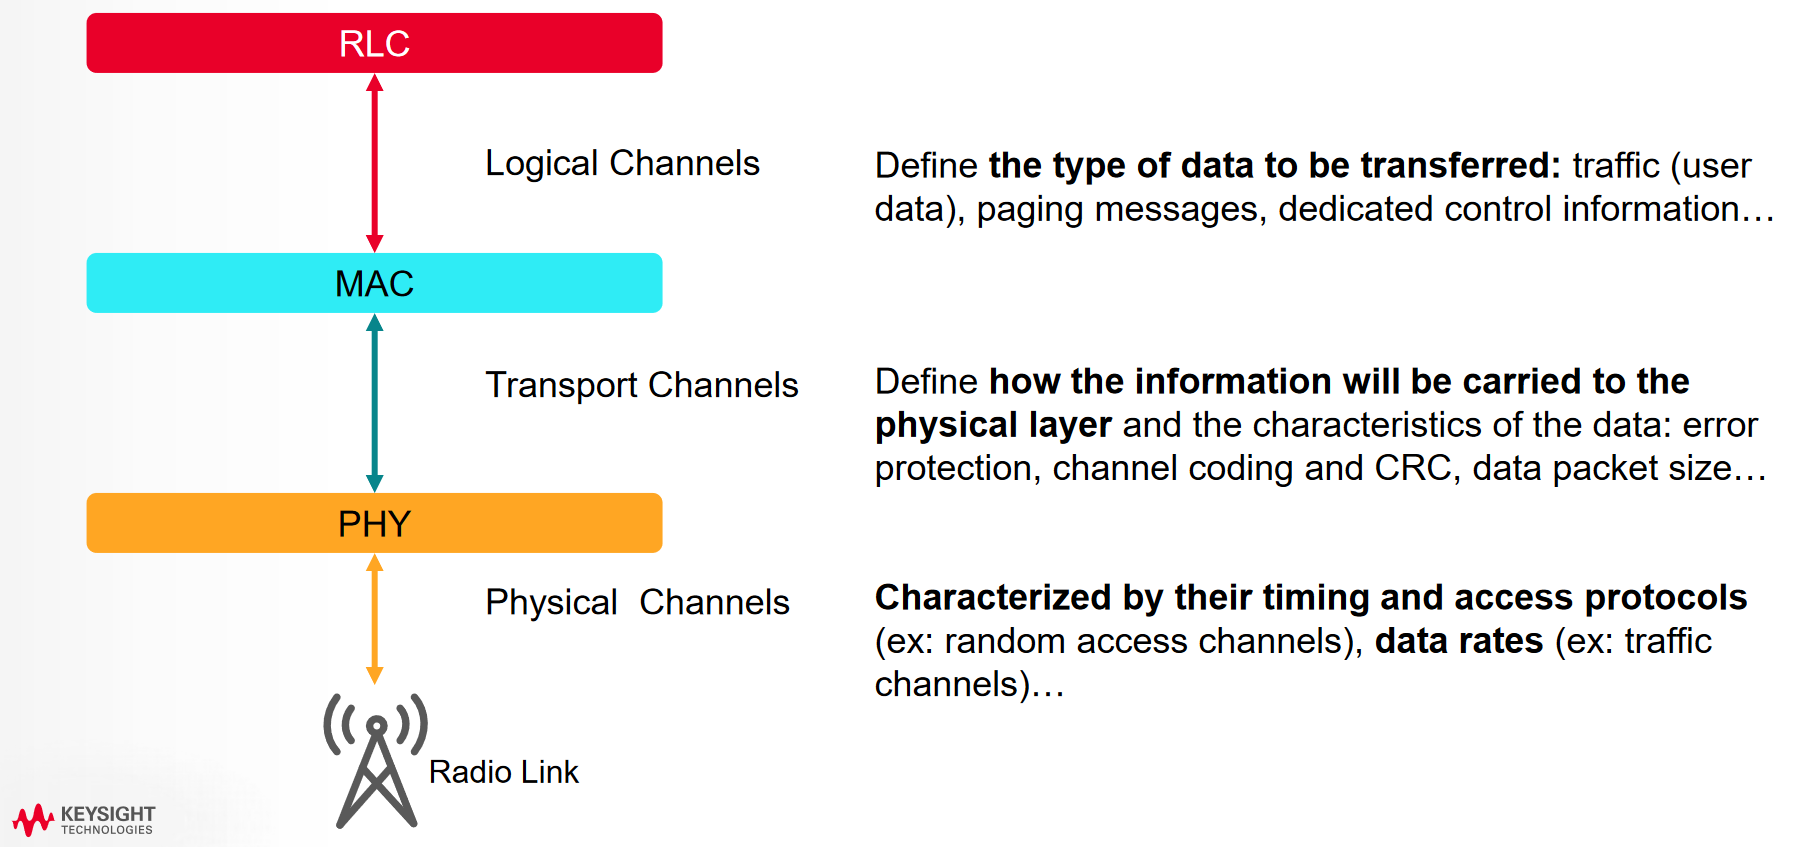
\includegraphics[width=0.9\textwidth]{res/nr-types-channels.png}
    \caption{Different types of channels used in 5G, courtesy of \href{https://www.keysight.com/}{ Keysight technologies}}
    \label{fig:nr-types-channels}
\end{figure}

\subsection{TDD operation}
The most complex problem to solve when dealing with propagation delay is certainly the \ac{TDD} mode of operation. In this scenario, each user can communicate only inside its assigned time slots.

Differently from 4G, where a predefined pattern was in place when allocating downlink and uplink allocations in a radio frame, in New Radio this is done much more flexibly using a plethora of parameters such as the periodicity of UL and DL transmissions, the number of consecutive DL and UL slots and symbols at the beginning of each pattern and more.

\paragraph{}The important key concept is that all the scheduler work has to account for the propagation delay. While in terrestrial communications guard periods of six symbols when switching from downlink communications to uplink communications is sufficient to account for the delay in a 32Km-radius cell, and timing advance commands can account for the different propagation delays experienced by users located in the center of the cell and users located in the cell edge \cite{gsma-5g-tdd-sync}, the same cannot be said for non-terrestrial use cases, where the distances that come into play are much longer, therefore any delay is orders of magnitude higher.

\section{Accounting for propagation delay in scheduling}

\subsection{Problem description}
\label{ss:propdelay-problem-desc}
\paragraph{}
The first encountered problem while implementing a non-terrestrial communication scenario in the simulator was the inability of the scheduler to account for the propagation delay when allocating radio resources to the connected user equipment on the ground.

The implementation of the 5G scheduler in ns-3 is designed to allocate resources less than a single subframe in advance, and since each subframe has a duration time of 1ms, the resource grant was already expired by the time it was able to reach the \ac{UE}, since it was referring to a past subframe.

\paragraph{Example} Consider a scenario with a propagation delay $\tau_p$ of 6ms. The \ac{UE} sends a request for uplink resources at time $t_0$ since it has some data to send. In the terrestrial scheduler implementation, the \ac{gNB} would receive such request at $t_0+\tau_p=6\textit{ms}$ and, provided that other transmissions have not been scheduled yet, grant the \ac{UE} the possibility to transmit in the following slot, which will start after 1ms at $t_0+\tau_p+t_{\textit{slot}}=7\textit{ms}$. However, this grant will reach the \ac{UE} only after another propagation delay, therefore at $t_0+2\tau_p=12\textit{ms}$, when it will already be too late.

\subsection{Proposed solution}
The implemented solution assumes that the scheduler has knowledge of the propagation delay. This is a reasonable assumption since systems such as GPS already rely on a precise estimation of the delay between the user on the ground and the satellite.

The scheduling then proceeds as normal with the only difference being that the information regarding the propagation delay is used to postpone the allocated symbols. 

\paragraph{Example} Consider the same scenario of the previous example in section \ref{ss:propdelay-problem-desc}. The new implementation of the scheduler accounts for the propagation delay by allocating the first available slot after $\tau_p$, so the time for the grant to reach the \ac{UE} is accounted for, and the \ac{gNB} marks the slot after $2\tau_p$ as reserved.

The last part of reserving a different slot is not as immediate. However, this mechanism needs to be in place because of the behavior depicted in Figure \ref{fig:scheduler-allocations-pd}, where a scenario with propagation delay of 5 slots (roughly 1,2ms) is considered:


\begin{itemize}
    \item \ac{UE} sends the scheduling request to \ac{gNB} at frame 1, subframe 0, slot 0.
    \item The \ac{SR} reaches the \ac{gNB} after $1\tau_p$ of 5 slots and the \ac{UE} is scheduled to transmit at frame 1, subframe 2, slot 2 since there is some noticeable propagation delay.
    \item The \ac{SR} reaches the \ac{UE} at frame 1, subframe 2, slot 2, and the \ac{UE} can transmit right away.
    \item The packet reaches the \ac{gNB} after another $\tau_p$, hence the base station needs to know that it cannot schedule other transmissions to take place in this slot, otherwise interference and collisions may arise.
\end{itemize}

\begin{figure}[ht]
    \centering
    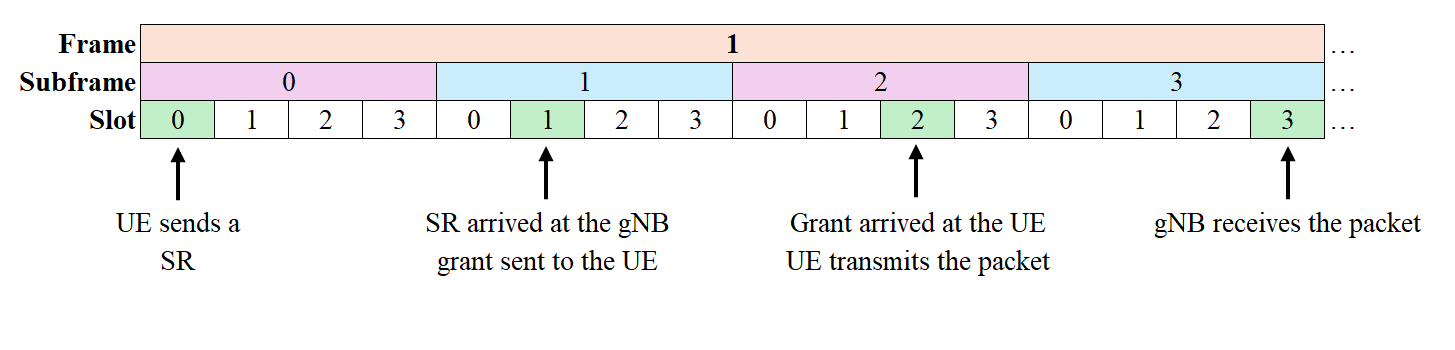
\includegraphics[width=0.9\textwidth]{res/scheduler-allocation-pd.png}
    \caption{Difference between allocated slot and gNB reception}
    \label{fig:scheduler-allocations-pd}
\end{figure}

\section{BSR timer}

After implementing the solution of the previous point in the ns-3 network simulator allowing the communication to take place, some other irregularities were found.
In particular, the 
\todo{Describe how the BSR automatic timeout was discovered, the problem, show the plots in fixed\_distance\_si10\_udp both the physical layer and the e2e throughput, highlighting the difference. Tell how this was fixed increasing the timer. It has to account at least for 2*tp. This is detailed in section 5.4.5 of https://www.etsi.org/deliver/etsi\_ts/138300\_138399/138321/18.01.00\_60/ts\_138321v180100p.pdf}

\section{Inflated BSR}

\todo{Describe the mechanism whenever the send interval was smaller than an RTT, leading to bigger BSR so bigger grants, a lower latency but also some wasted capacity. }

\section{Reordering timer}

\todo{The misalignment between the send interval and the propagation delay leads to the sending of fragmented packets since the grants are always a bit bigger than the packet UE has to send. However, the gNB reordering timer is configured for terrestrial networks, so it expires before we have a chance of receiving the full picture.}
    %!TEX root = ../main.tex

\chapter{HARQ}
\label{chp:harq}

\section{HARQ overview}
The main objective of telecommunication technologies is the transfer of information between different actors. Modern systems aim at an efficient usage of the available resources, while trying to meet all the necessary requirements of the application that is generating the data to be transferred. 

The \ac{HARQ} protocol hereby described helps achieve a more efficient use of the available resources when errors occur, using an intelligent system of retransmissions that, in turn, lowers the error rate at the expense of a higher latency.

The main building blocks of \ac{HARQ} are \ac{ARQ} and \ac{FEC}. The role of \ac{ARQ} is to automatically request the retransmission of the whole packet when the receiver detects the presence of errors, while \ac{FEC} is tasked to correct such errors using redundancy bits added to the packet by the transmitter. The joint operation of those two protocols makes the foundation of \ac{HARQ}, currently in use in all the most popular network standards such as 4G, Wi-Fi and 5G \cite{3gpp-38-series}. \ac{HARQ} peculiarity resides in the fact that it avoids the retransmission of the whole packet in case of errors, preferring to send additional redundant information to help the decoding process.

\section{Concurrent processes limit}
\label{sec:harq-conc-proc}

One of the problems highlighted by the \ac{3GPP} technical report \cite{3gpp-tr-38.811} on the matter of non-terrestrial networks regards the maximum number of concurrent \ac{HARQ} processes. 

\subsection{Problem description}
The details of \ac{HARQ} protocol implementation in the 5G \ac{NR} standard is extensively treated in many publications such as \cite{harq-wireless-communications-survey}. However, for the purpose of understanding what is a \ac{HARQ} process and how it affects the throughput in a non-terrestrial scenario, a brief overview of a few key concepts is enough.

\begin{figure}[ht]
    \centering
    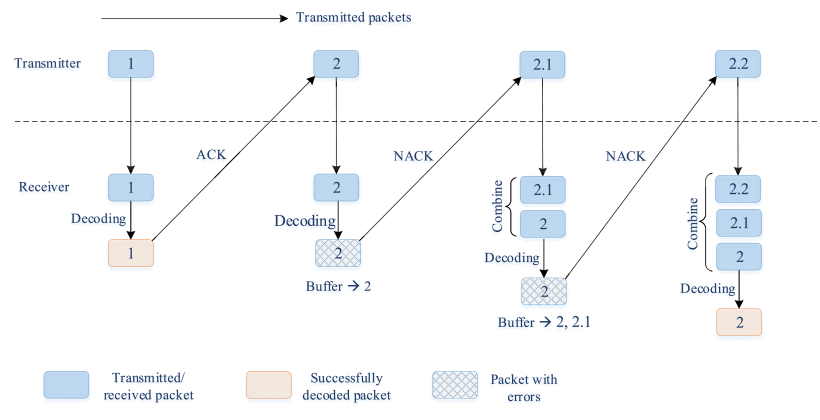
\includegraphics[width=0.9\textwidth]{res/harq-retx-scheme.png}
    \caption{\ac{HARQ} retransmission diagram \cite{harq-wireless-communications-survey}}
    \label{fig:harq_retx_scheme}
\end{figure}

\subsubsection{HARQ working principle}
\paragraph{}
Fig. \ref{fig:harq_retx_scheme} gives an overview of how \ac{HARQ} processes work. Upon successful reception, depicted in the first column of Fig. \ref{fig:harq_retx_scheme}, an \ac{ACK} is sent back, triggering the transmission of the successive \ac{TB}, which is represented in the second column. This behavior is the normal state in which transmissions are received correctly, and it keeps repeating itself until errors are detected.

\paragraph{} Should the receiver detect errors in the received \ac{TB}, represented by the greyed packet, a \ac{NACK} is relayed back to the sender, which in turn proceeds to send some additional redundancy bits. Note that the sender does not repeat the whole \ac{TB}. The receiver now proceeds to decode the transfer block using all the information that it has received so far.

This is the most important feature of \ac{HARQ} protocol: it does not discard the packets affected by errors, since they can be at least used to recover some information. The erroneous packets are stored in buffers and used for joint decoding \cite{5g-nr-harq-devopedia}. 

\paragraph{} If the redundancy bits that the sender just transmitted are still not enough to allow for a correct decoding of the transfer block, or if another error is detected, a retransmission is triggered. This is shown in the last column of Fig. \ref{fig:harq_retx_scheme}, where all the packets received so far contribute in correctly decoding packet 2.

Finally, if even this retransmission is affected by errors and the combination of the information received so far is not enough to complete the decoding of the \ac{TB}, additional information is sent. After this fourth interaction, no further attempts are made to correct the packet \cite{5g-nr-harq-sharetechnote}.

\paragraph{} The various transmissions and retransmissions being made by the protocol are called \ac{RV}, and are numbered from 0 to 3. Their order can vary depending on the implementation and configuration. Figure \ref{fig:harq_retx_scheme_2} shows another example where the redundancy versions are ordered as 0, 3, 2.

\begin{figure}[ht]
    \centering
    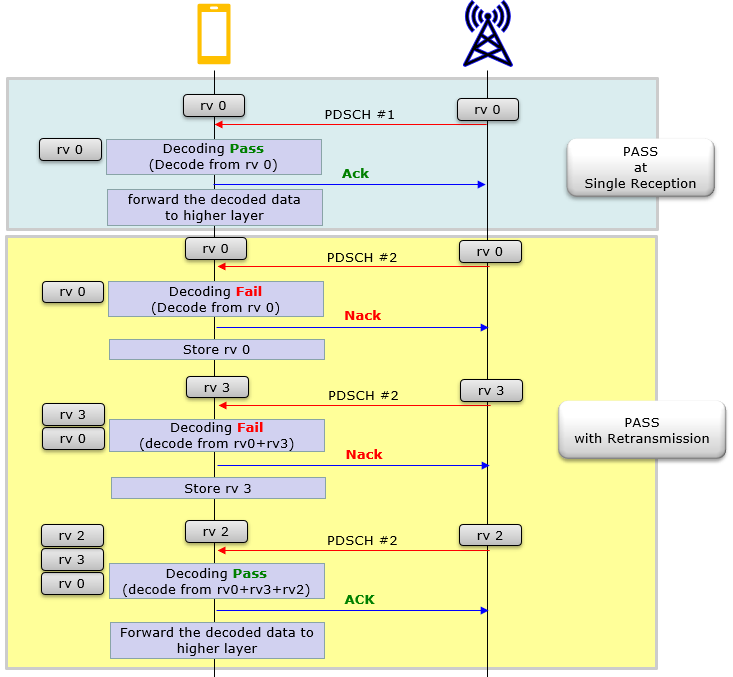
\includegraphics[width=0.9\textwidth]{res/harq-retx-scheme-2.png}
    \caption{\ac{HARQ} diagram with different RVs\cite{5g-nr-harq-sharetechnote}}
    \label{fig:harq_retx_scheme_2}
\end{figure}


\subsubsection{Stop and wait}
\paragraph{} The presented behavior means that \ac{HARQ} is a stop-and-wait kind of protocol, since it is designed to wait for the arrival of previous packet's \ac{ACK} before sending the new one. While this enforces the delivery of ordered packets, it also brings the downside of severely underutilizing the channel capacity, wasting resources that could potentially be used for transmission instead \cite{3gpp-ts-38.214}. Figures \ref{fig:harq_retx_scheme_2} and \ref{fig:harq_retx_scheme} highlight this pattern.

This limitation is overcome by the introduction of multiple concurrent processes.

\subsubsection{Processes}
\paragraph{}
A \ac{HARQ} process starts when a \ac{TB} is passed to the \ac{HARQ} entity and finishes when the \ac{ACK} relative to that same \ac{TB} is received by the sender. After the \ac{ACK} is correctly received, the next \ac{TB} starts being processed. Considering a link with propagation delay $\tau_p$, the minimum active time for a process is therefore $2\tau_p$, i.e. the time for the transfer block to arrive to the destination plus the time for the acknowledgement to travel back to the sender.

The 5G \ac{NR} standard allows the base station to configure the maximum number of concurrent \ac{HARQ} processes to be assigned to each connected user, with the default value being of 8 concurrent processes and the maximum 16 \cite{3gpp-ts-38.300, 5g-nr-harq-devopedia}. In this way it is possible to partially limit the effects of the stop-and-wait behavior, allowing for a better throughput.

\subsubsection{Application in NTNs}
\paragraph{}
Since the propagation delay of \ac{NTNs} is order of magnitude larger than their terrestrial counterpart, the limited maximum number of concurrent processes lowers the maximum achievable throughput, as detailed in the following toy example. 

\paragraph{Example} Consider a scenario where each process tries to send a \ac{TB} every $2\tau_p$, which is the maximum rate at which transfer blocks can be sent under the condition of waiting for the acknowledgement to arrive before starting a new transmission. The other endpoint is a \ac{LEO} satellite orbiting at 2.000Km, therefore having $\tau_p\approx6$ms. Assuming the best possible conditions with no need for retransmissions and assuming that the base station grants the \ac{UE} to the best possible clearance of 16 concurrent processes, the total send rate is of 16 transfer blocks every 12ms. In order to target a throughput of 50Mbps, the block size must therefore be of at least $$\frac{\textit{target throughput} \times 2\tau_p}{\textit{number of processes}} = 37,5Kb$$
Doing the same calculation for a terrestrial scenario with the \ac{gNB} placed at a distance of 600m from the \ac{UE}, we obtain that the minimum \ac{TBS} must be of just $12b$.
Both calculations do not factor in overheads, control information, channel access requests and processing delays, but are helpful to give an idea of the disproportion in place between the two conditions.

While the necessary block size for the \ac{NTN} case is technically possible to achieve even with the older 4G technology, it necessitates a high \ac{SNR} to work properly. This constraint becomes even more conservative in the non-terrestrial case, since retransmissions add delays in multiples of the propagation delay and can therefore quickly become a lot more costly \cite{4g-phy-processing-sharetechnote}.

\subsection{Possible solutions}
\label{sec:proc-harq-prop-sol}
\paragraph{Increasing the processes}
The easiest solution would be to increase the number of maximum concurrent \ac{HARQ} processes. However, this comes with some caveats mainly regarding the higher computational capabilities required and higher power consumption, that can quickly become problematic in battery-operated equipments such as smartphones. Each process also requires the presence of a buffer on both the receiver side and the sender side, so additional resources are required at the \ac{gNB}, too. 
\paragraph{Aggressive HARQ}
A more sophisticated approach could involve the design of an aggressive version of the \ac{HARQ} protocol, where each process is allowed to send multiple packets before receiving an acknowledgement. Since there already are multiple concurrent processes, each \ac{ACK} packet must already contain a field specifying the number of process it belongs to, and the information identifying the specific packet to be acknowledged within a process could be encoded inside this field.
\paragraph{Disable \ac{HARQ}}
Lastly, the option of disabling \ac{HARQ} completely and rely solely on \ac{ARQ} retransmissions has been proposed by 3GPP itself \cite{hybrid-arq-schemes-muk}. This, however, would come with a performance penalty since satellite links typically suffer from more severe conditions than terrestrial ones, and \cite{5g-beyond-5g-ntn-trends-vanellicoralli} demonstrated that a version of \ac{HARQ} specifically designed for non-terrestrial networks would be beneficial.

\subsection{Implemented solution - More processes}
\subsubsection{Testing current implementation}
\paragraph{}
To test the practical effect that the concurrent processes' limitation has on the achievable throughput, a simulation campaign was conducted where the \ac{HARQ} protocol was firstly disabled and successively enabled, therefore obtaining results for the two different scenarios. The maximum number of concurrent processes with \ac{HARQ} enabled was set to 16, that is the maximum that a \ac{gNB} can allocate to each \ac{UE}.

\paragraph{}
Comparing the obtained results confirmed that employing \ac{HARQ} caused a noticeable negative impact on the throughput, as can be appreciated in Fig. \ref{fig:harq_on_off}. The throughput without \ac{HARQ} perfectly matches the source rate, since the \ac{SNR} values of this simulation are high enough to correctly deliver almost the totality of the packets. 

On the other hand, the throughput with \ac{HARQ} enabled reaches its plateau as the source rate crosses the 4Mb/s threshold, settling at this value. \ac{HARQ} struggles to keep up with the increasing source rate since the limited number of processes starts to cause packets to be dropped whenever a retransmission is needed. For a high enough source rate, the \ac{HARQ} protocol is completely overwhelmed, as all the 16 processes are always busy, and the arriving packets that do not find an available process are promptly discarded.


\begin{figure}[ht]
    \centering
    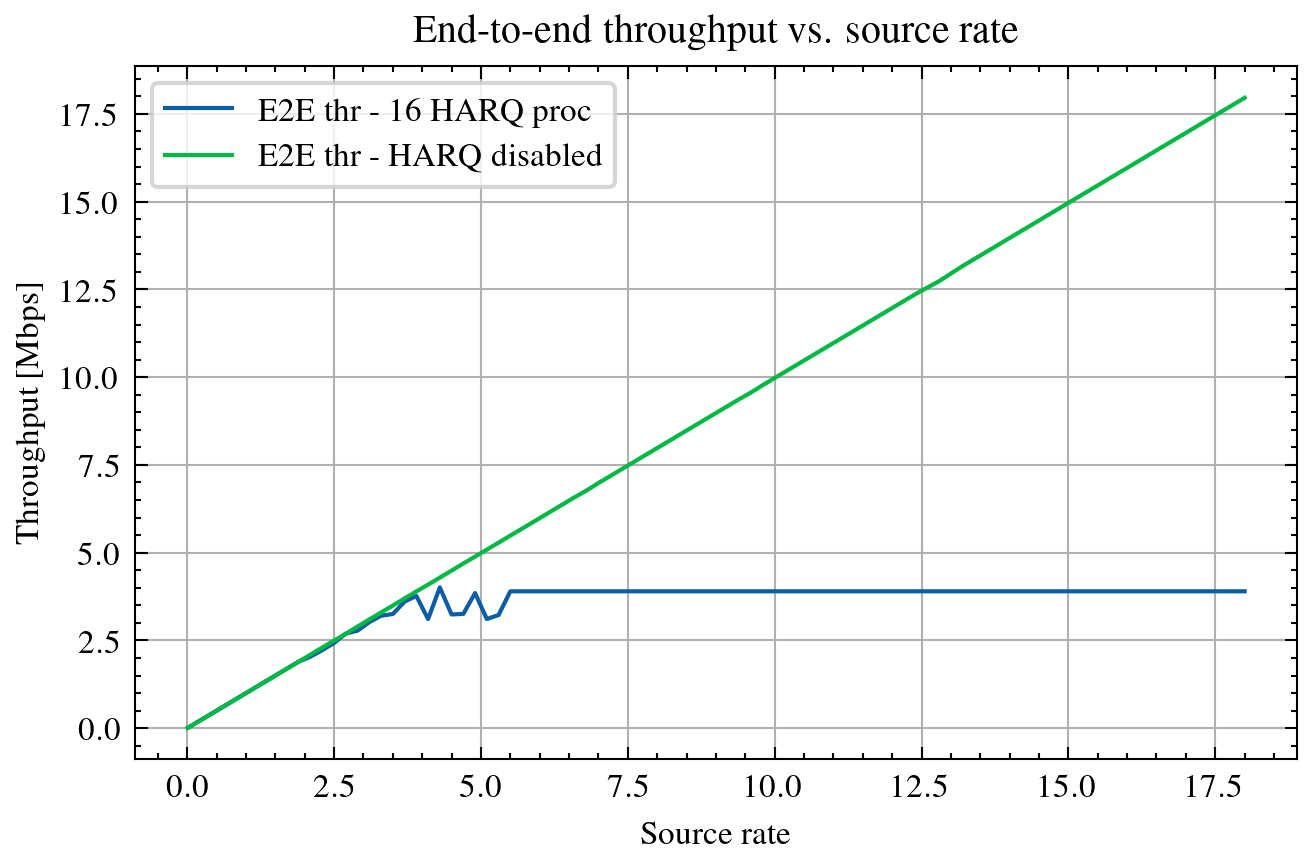
\includegraphics[width=0.9\textwidth]{res/harq-onoff2.png}
    \caption{End-to-end throughput comparison with and without \ac{HARQ}, $\tau_p=6$ms.}
    \label{fig:harq_on_off}
\end{figure}

\paragraph{}
Having verified that \ac{HARQ} does indeed limit the achievable throughput, a modification was implemented to the protocol suite to manually force a higher number of concurrent processes. The simulation campaign was then re-run and the results are shown in Fig. \ref{fig:harq-numproc}.

\begin{figure}[ht]
    \centering
    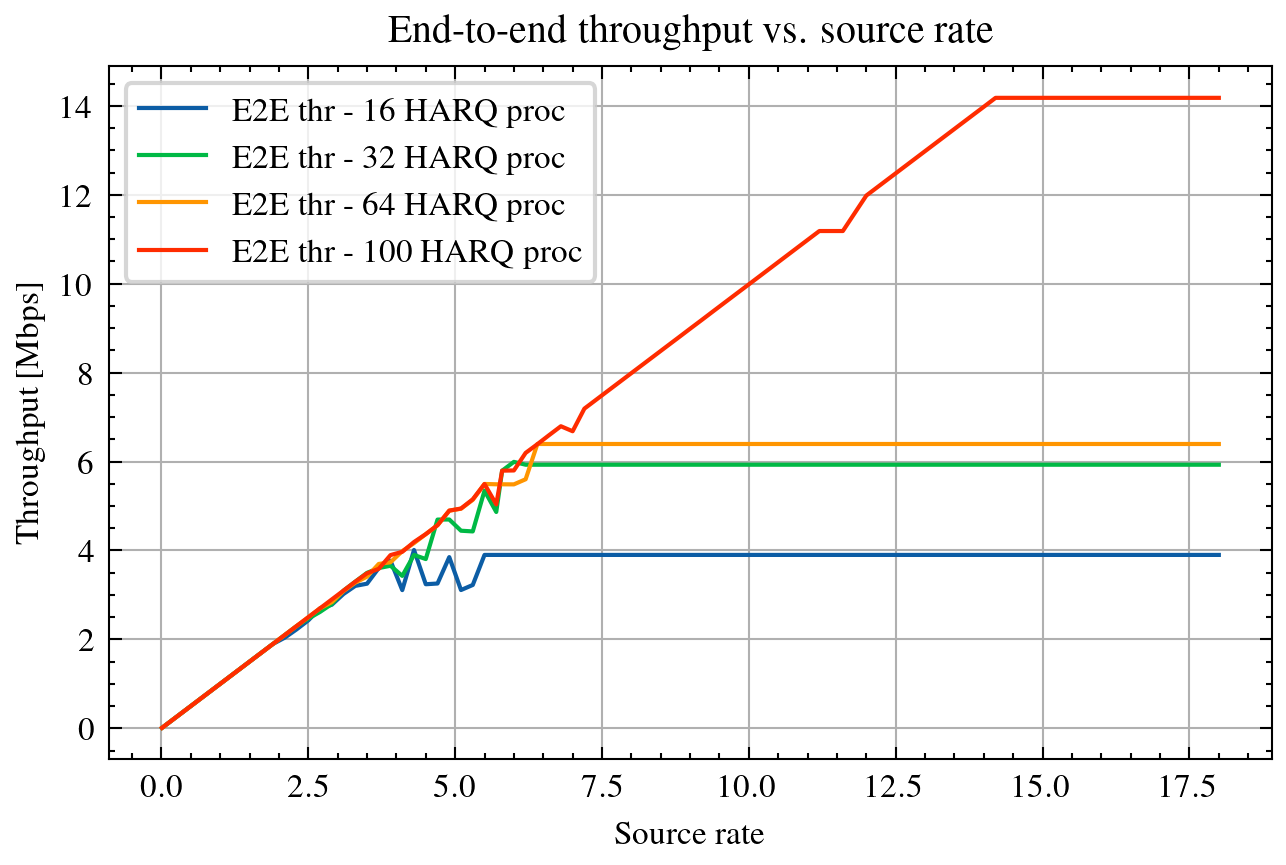
\includegraphics[width=0.9\textwidth]{res/harq_numproc_new.png}
    \caption{End-to-end throughput comparison with different number of concurrent \ac{HARQ} processes, $\tau_p=6$ms.}
    \label{fig:harq-numproc}
\end{figure}

\subsubsection{Results}
\paragraph{}
Increasing the allowed processes pushed the maximum achievable throughput to just over 14Mb/s in the scenario with the highest allowance of per-user concurrent processes. Going past such threshold causes packets to start being dropped, and the throughput to saturate, since there are no more available processes to send the traffic generated by the application.

The results shown in figure \ref{fig:harq-numproc} make clear that increasing the parameter regulating the number of \ac{HARQ} processes allows for higher speeds. Each line in the plot was obtained with a different number of allowed processes, starting from 16, the maximum allocable value in the 5G \ac{NR} standard, then 32, 64 and ultimately 100. No further increases have been evaluated, since those would currently be unrealistic to achieve.

However, constraints regarding the required computational power and the increased energy consumption shall also be taken into careful consideration, since raising the number of concurrent processes from 16 to 100 is a big step, bringing a consistent increase in both the receiver and transmitter complexity with it.

We can conclude that, while certainly being a way to improve the performances of \ac{HARQ} in non-terrestrial scenarios, the increase in processes alone cannot solve the problem of \ac{HARQ} limiting the throughput, therefore other ways have to be found, and future studies should also consider alternative proposals.

\subsection{Implemented solution - Disabling HARQ}
\paragraph{}
Figure \ref{fig:harq_on_off} could suggest that completely disable the \ac{HARQ} protocol could be a viable solution, since the end to end throughput of the simulation with \ac{HARQ} switched off always matched the source rate, meaning that all the packets generated by the application were correctly received by the remote host.

However, the reason of this behavior is the high \ac{SNR} that was forced in the simulated scenario with the choice of using high gain antennas. This design choice is not fully realistic, since the intended final use case of non-terrestrial networks is their usage with mobile handsets. Such choice was made because this work is focused on the study of the propagation delay, and the high gain of aperture antennas allowed to limit the impact of the problems caused by low \ac{SNR}. Having a communication channel with high \ac{SNR} allowed for fewer variables to impact the simulations' results, in turn enabling the study of propagation delay alone.

\paragraph{}
In order to test the performances without \ac{HARQ} enabled, a new simulation campaign has been conducted factoring in the problems related to poor \ac{SNR}, such as the presence of errors in the received packets and the need for retransmissions. In conditions of low \ac{SNR}, which can be plausible in a non-terrestrial communication scenario, the \ac{PDR} and therefore the throughput can drop considerably, impacting the link reliability.
\paragraph{}
Simulations have shown that fully disable \ac{HARQ} may be a good solution only when both \ac{UE} and \ac{gNB} experience optimal channel conditions with high \ac{SNR}, while poor channel conditions may benefit from having \ac{HARQ} enabled.

A hybrid approach can also be thought, where \ac{CQI} can be used to assess the state of the channel and decide whether to enable \ac{HARQ}, therefore limiting the throughput in exchange for a higher reliability, or disabling it, should the \ac{SNR} be high enough.

\iffalse
    \subsection{Simulator configuration}
    While the number of concurrent HARQ processes can be configured in ns-3, it cannot exceed the value of 100. By performing some simple calculations, knowing that the \ac{SNR} conditions allow for the transmissions of \ac{TB}s with size of 1024B, to achieve a target throughput of 50Mbps on the best case of 6ms $\tau_p$ the necessary processes would be 74.
    $$\frac{\textit{target throughput} \times 2\tau_p}{\textit{total block size}} \approx 74 \textit{processes}$$

    This does not account for the delays caused by retransmissions, so simulator crashes due to processes overflow are frequent while testing even the best case scenario.

\fi


    %!TEX root = ../main.tex

\chapter{Conclusions and Future Works}
\label{chp:conclusions}

This work has provided a comprehensive study on the impact that the high propagation delay experienced in \ac{NTN}s has in layer-2 protocols. The current codebase of the ns-3 network simulator has been properly extended to allow for end-to-end simulation of the \ac{NR} stack in a \ac{NTN} scenario, since the ns-3 implementation of \ac{NR} technology was not designed for high propagation delays. A lot of work went therefore into the design, implementation, and testing of a base support for the simulation of \ac{NTN}s.

It was shown that propagation delay plays a crucial role in the performances of \ac{NR} in \ac{NTN}s, affecting both the efficiency and reliability of data transmission.

\paragraph{}
Once the simulator was ready, focus has been placed on the optimization of the \ac{HARQ} protocol in \ac{NTN}s, investigating its shortcomings when delaing with large propagation delays as well as proposing some original solutions to increase its performances.

\section{Results}
\subsection{Simulator redesign}
Since the state of the art in network simulation tools was not ready for complete \ac{NR} \ac{NTN} simulations, presenting numerous problems especially at the scheduler, a redesign of certain behaviors was performed.

\subsubsection{Scheduling with propagation delay}
This study has found (section \ref{sec:pd-sched-acc}) that the current scheduling with short advance (i.e. scheduling only a slot in advance: at time $t_0$ the schedule allocates the resources of time $t_0+1$ms) does not work in \ac{NTN} because the propagation delay itself is longer than the delay between the act of scheduling and the time for which the scheduling happens. 

The proposed solution uses information on the propagation delay to adjust the advance of the scheduling process. 

\subsubsection{BSR timer}

Another flaw discovered in the implementation of current \ac{NR} protocols in \ac{NTN} involves the periodic \ac{BSR} that the \ac{UE} keeps sending every 10ms (section \ref{sec:bsr-timer}). 

While this approach presents some (undesired) benefits, it is not the intended behavior, therefore the current implementation, albeit working, is far from an ideal choice.

The proposed solution consists of adapting the \ac{BSR} timer accordingly to the propagation delay, never allowing it to assume values smaller than a round-trip time. 

\subsubsection{Inflated BSR}
If the interval between the packets generated by the application is smaller than the \ac{RTT}, each \ac{BSR} will report the whole size of the transmission buffer, even though other \ac{SR} relative to packets already present in the buffer may be still in-flight. While leading to an overall lower latency, this vastly increases the amount of resources being wasted, since the \ac{UE} will find itself with many unnecessary transmission grants (Section \ref{sec:inf-bsr}).

The proposed solution is to limit the scheduling requests that are triggered every time a packet arrives into the transmission buffer to the new data only.

\subsubsection{Reordering timer}
The conducted simulation campaigns have found that anytime a packet is fragmented and sent across multiple frames, a reordering and recomposition timer is activated at the \ac{gNB} side, which, however, is too short with respect to the large propagation delay in \ac{NTN}s, expiring before all the pieces of the packet have the chance to arrive (Section \ref{sec:reord-timer}).

The implemented solution was to extend such timer in order to account for the propagation delay.

\subsection{HARQ}
\subsubsection{Concurrent processes}
This work confirmed that the 16 maximum concurrent \ac{HARQ} processes allowed per user heavily limits the achievable throughput (section \ref{sec:harq-conc-proc}).

Different solutions have been proposed, including completely disabling the protocol as well as increasing the number of allowed concurrent processes.

Both these solutions have also been implemented in the simulator, evaluating scenarios with no \ac{HARQ}, then 16, 32, 64 and 100 maximum concurrent processes. 

It was found that increasing the number of processes allows for considerably higher throughputs, while disabling \ac{HARQ} is only feasible in conditions of high \ac{SNR}.

Since having \ac{HARQ} enabled still proved to be helpful in a scenario of low \ac{SNR}, a more aggressive version of \ac{HARQ} was designed, where each process was allowed to send two packets instead of one before waiting for the \ac{ACK}. This solution managed to roughly double the achievable throughput with respect to the standard \ac{HARQ} implementation.

\section{Future work}

The preparation of this work required many simulations to be run and evaluated, and as expected some design problems emerged. With a thoughtful approach, each unexpected behavior was investigated and solutions were devised, implemented and tested.

While effort was made to provide more than a single solution, striving to look at the problems from different perspectives to find more than a single way to approach it, some possibilities still require a deeper study, and some observations were made whenever it was felt that a point might benefit from additional work.

This section describes some possible future paths that might have the potential to improve the solutions proposed in this work, as well as different approaches which performances are still to be evaluated.

\paragraph{}
The current behavior of waiting for packets to arrive at the transmission buffer of the \ac{UE} before transmitting the \ac{SR} to the \ac{gNB} harshly impacts the experienced latency, since in the best-case scenario it at least adds a round-trip time of delay. While this is not a problem in terrestrial networks because base stations are relatively close to the \ac{UE}s that are serving, in \ac{NTN}s the added delay is noticeable. 

A predictive algorithm capable of visualizing patterns in the \ac{UE}-generated traffic, forecasting its behavior in the immediate future and preemptively sending \ac{SR} so that new packets will be able to be transmitted right away without additional delays would be of invaluable help in reducing the overall latency of the link.

\paragraph{}
Timers often represent a trade-off between higher performances and a more robust network. This is the reason behind the proposal of a dynamic approach when setting the values for \ac{BSR} periodic requests and reordering timer. Since the delay of \ac{NTN}s can experience large variations depending on the satellite orbit, configurable timers shall be preferred instead of using fixed values.

\paragraph{}
Regarding \ac{HARQ}, a dynamic way of enabling and disabling it on the fly based on channel quality indicators could be beneficial, since it was shown that high-\ac{SNR} scenarios performed better with \ac{HARQ} disabled, while conditions of low \ac{SNR} benefitted from having it enabled.

\paragraph{}

It is clear that further research is needed to develop more effective strategies for managing propagation delay in \ac{NTN}s. This includes exploring new technologies, improving existing methodologies, and devising innovative network architectures.

Ultimately, this work aims to pave the way for future research and practical applications in the field of \ac{NTN}s, emphasizing the need for continuous innovation and adaptation to meet the evolving demands of modern communication systems. 

The findings of this thesis not only contribute to the existing body of knowledge on \ac{NTN}s but also pave the way for future research in this evolving field.

    
    % Bibliography, appendix, acknowledges, etc...
    \backmatter
\end{document}